\begin{figure*}[!htbp]
\begin{center}

  \begin{subfigure}[b]{0.5\linewidth}
    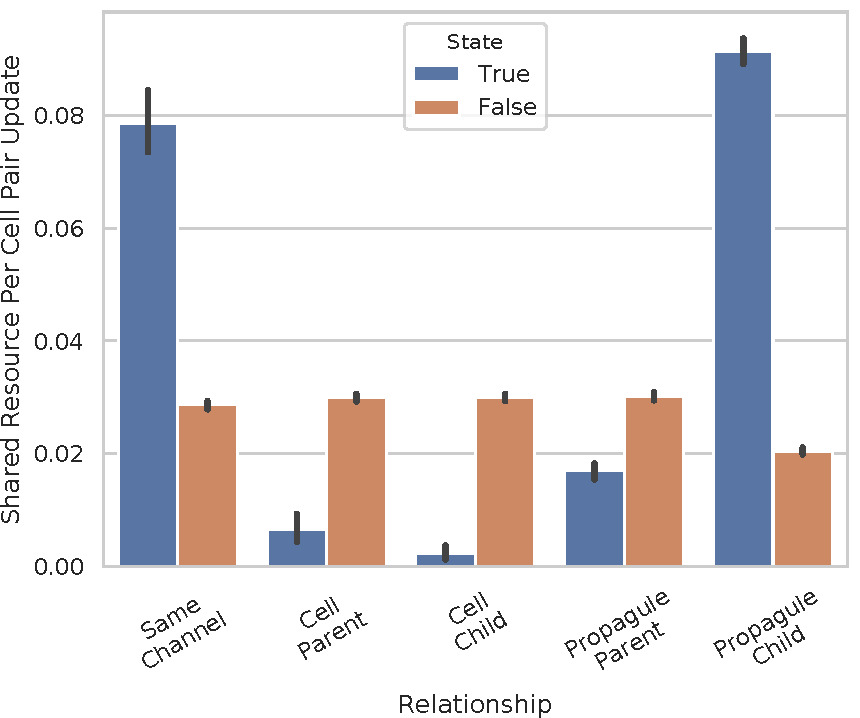
\includegraphics[width=\linewidth]{title=resource_contributed_start+treat=wave-big__mut-d_high+_data_hathash_hash=b9225de9509badc8+_script_fullcat_hash=064800f3ddff6753+_source_hash=d53f428-clean+ext=}
    \caption{Large Resource Wave, Mutational Load 4}
  \end{subfigure}

  \begin{subfigure}[b]{0.5\linewidth}
    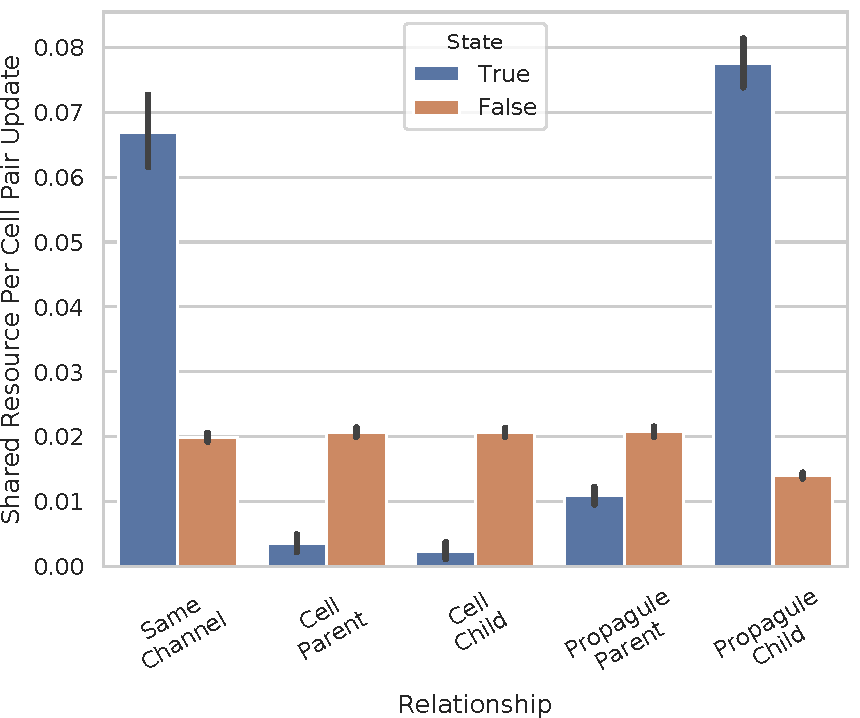
\includegraphics[width=\linewidth]{title=resource_contributed_start+treat=wave-big__mut-e_extreme+_data_hathash_hash=83586cb816dd102d+_script_fullcat_hash=064800f3ddff6753+_source_hash=d53f428-clean+ext=}
    \caption{Large Resource Wave, Mutational Load 5}
  \end{subfigure}

\caption{
Resource sharing phenotypes between updates 0 and 20 for high mutational load, large resource wave treatments.
Bar height represents the mean amount of resource transferred per update per neighboring pair of cells.
Each two-tone pair of bars compares cell pairs with a particular relationship to cell pairs without that relationship.
The ``Same Channel'' bar pair compares resource sharing between cell pairs with a common channel and cell pairs on different channels.
The ``Cell Parent'' bar pair compares the amount of resource shared from a cell to its cellular parent to the amount of resource shared from a cell to cells that are not its cellular parent.
The ``Cell Child'' bar pair compares the amount of resource shared from a cell to its cellular child to the amount of resource shared from a cell to cells that are not its cellular child.
For the next two relationships, consider a cell with channel ID $A$ that reproduces, producing a daughter cell with the new channel ID $B$.
Let the channel ID $C$ denote a channel ID that is unique from channel IDs $A$ and $B$.
The ``Propagule Parent'' bar pair compares the amount of resource shared from a cell to cells with the channel ID that its channel ID descends from (e.g., from cells with channel ID $B$ to cells with channel ID $A$) to the amount of resource shared to other cells that are not part of its same-channel network (e.g., to cells with channel ID $C$).
The ``Propagule Child'' bar pair compares the amount of resource shared from a cell to cells with a channel ID that descends from its channel ID (e.g., from cells with channel ID $A$ to cells with channel ID $B$) to the amount of resource shared to other cells that are not part of its same-channel network (e.g., to cells with channel ID $C$).
Error bars represent 95\% confidence intervals.
} \label{fig:resource_contributed_start}
\end{center}
\end{figure*}
